\subsection{CVSS TypeScript Implementation} \label{subsec:projektbericht-loesungsweg-typescript-cvss-online-calculator}

Dieses Kapitel geht auf die Details hinter der CVSS-Implementierung\footnote{\url{https://github.com/org-metaeffekt/metaeffekt-universal-cvss-calculator}} in TypeScript ein, wie sie im Universal CVSS Calculator\footnote{\url{https://www.metaeffekt.com/security/cvss/calculator}} der {\metaeffekt} verwendet wird.
In Abbildung \ref{fig:cvss-ts-calculator-class-diagram} kann das Klassendiagramm der TypeScript-Klassen mit allen Exports und Imports gefunden werden, welche in diesem Kapitel erklärt werden.

\begin{figure}[htbp] % here, top, bottom, separate page
    \centering
    \makebox[\textwidth][c]{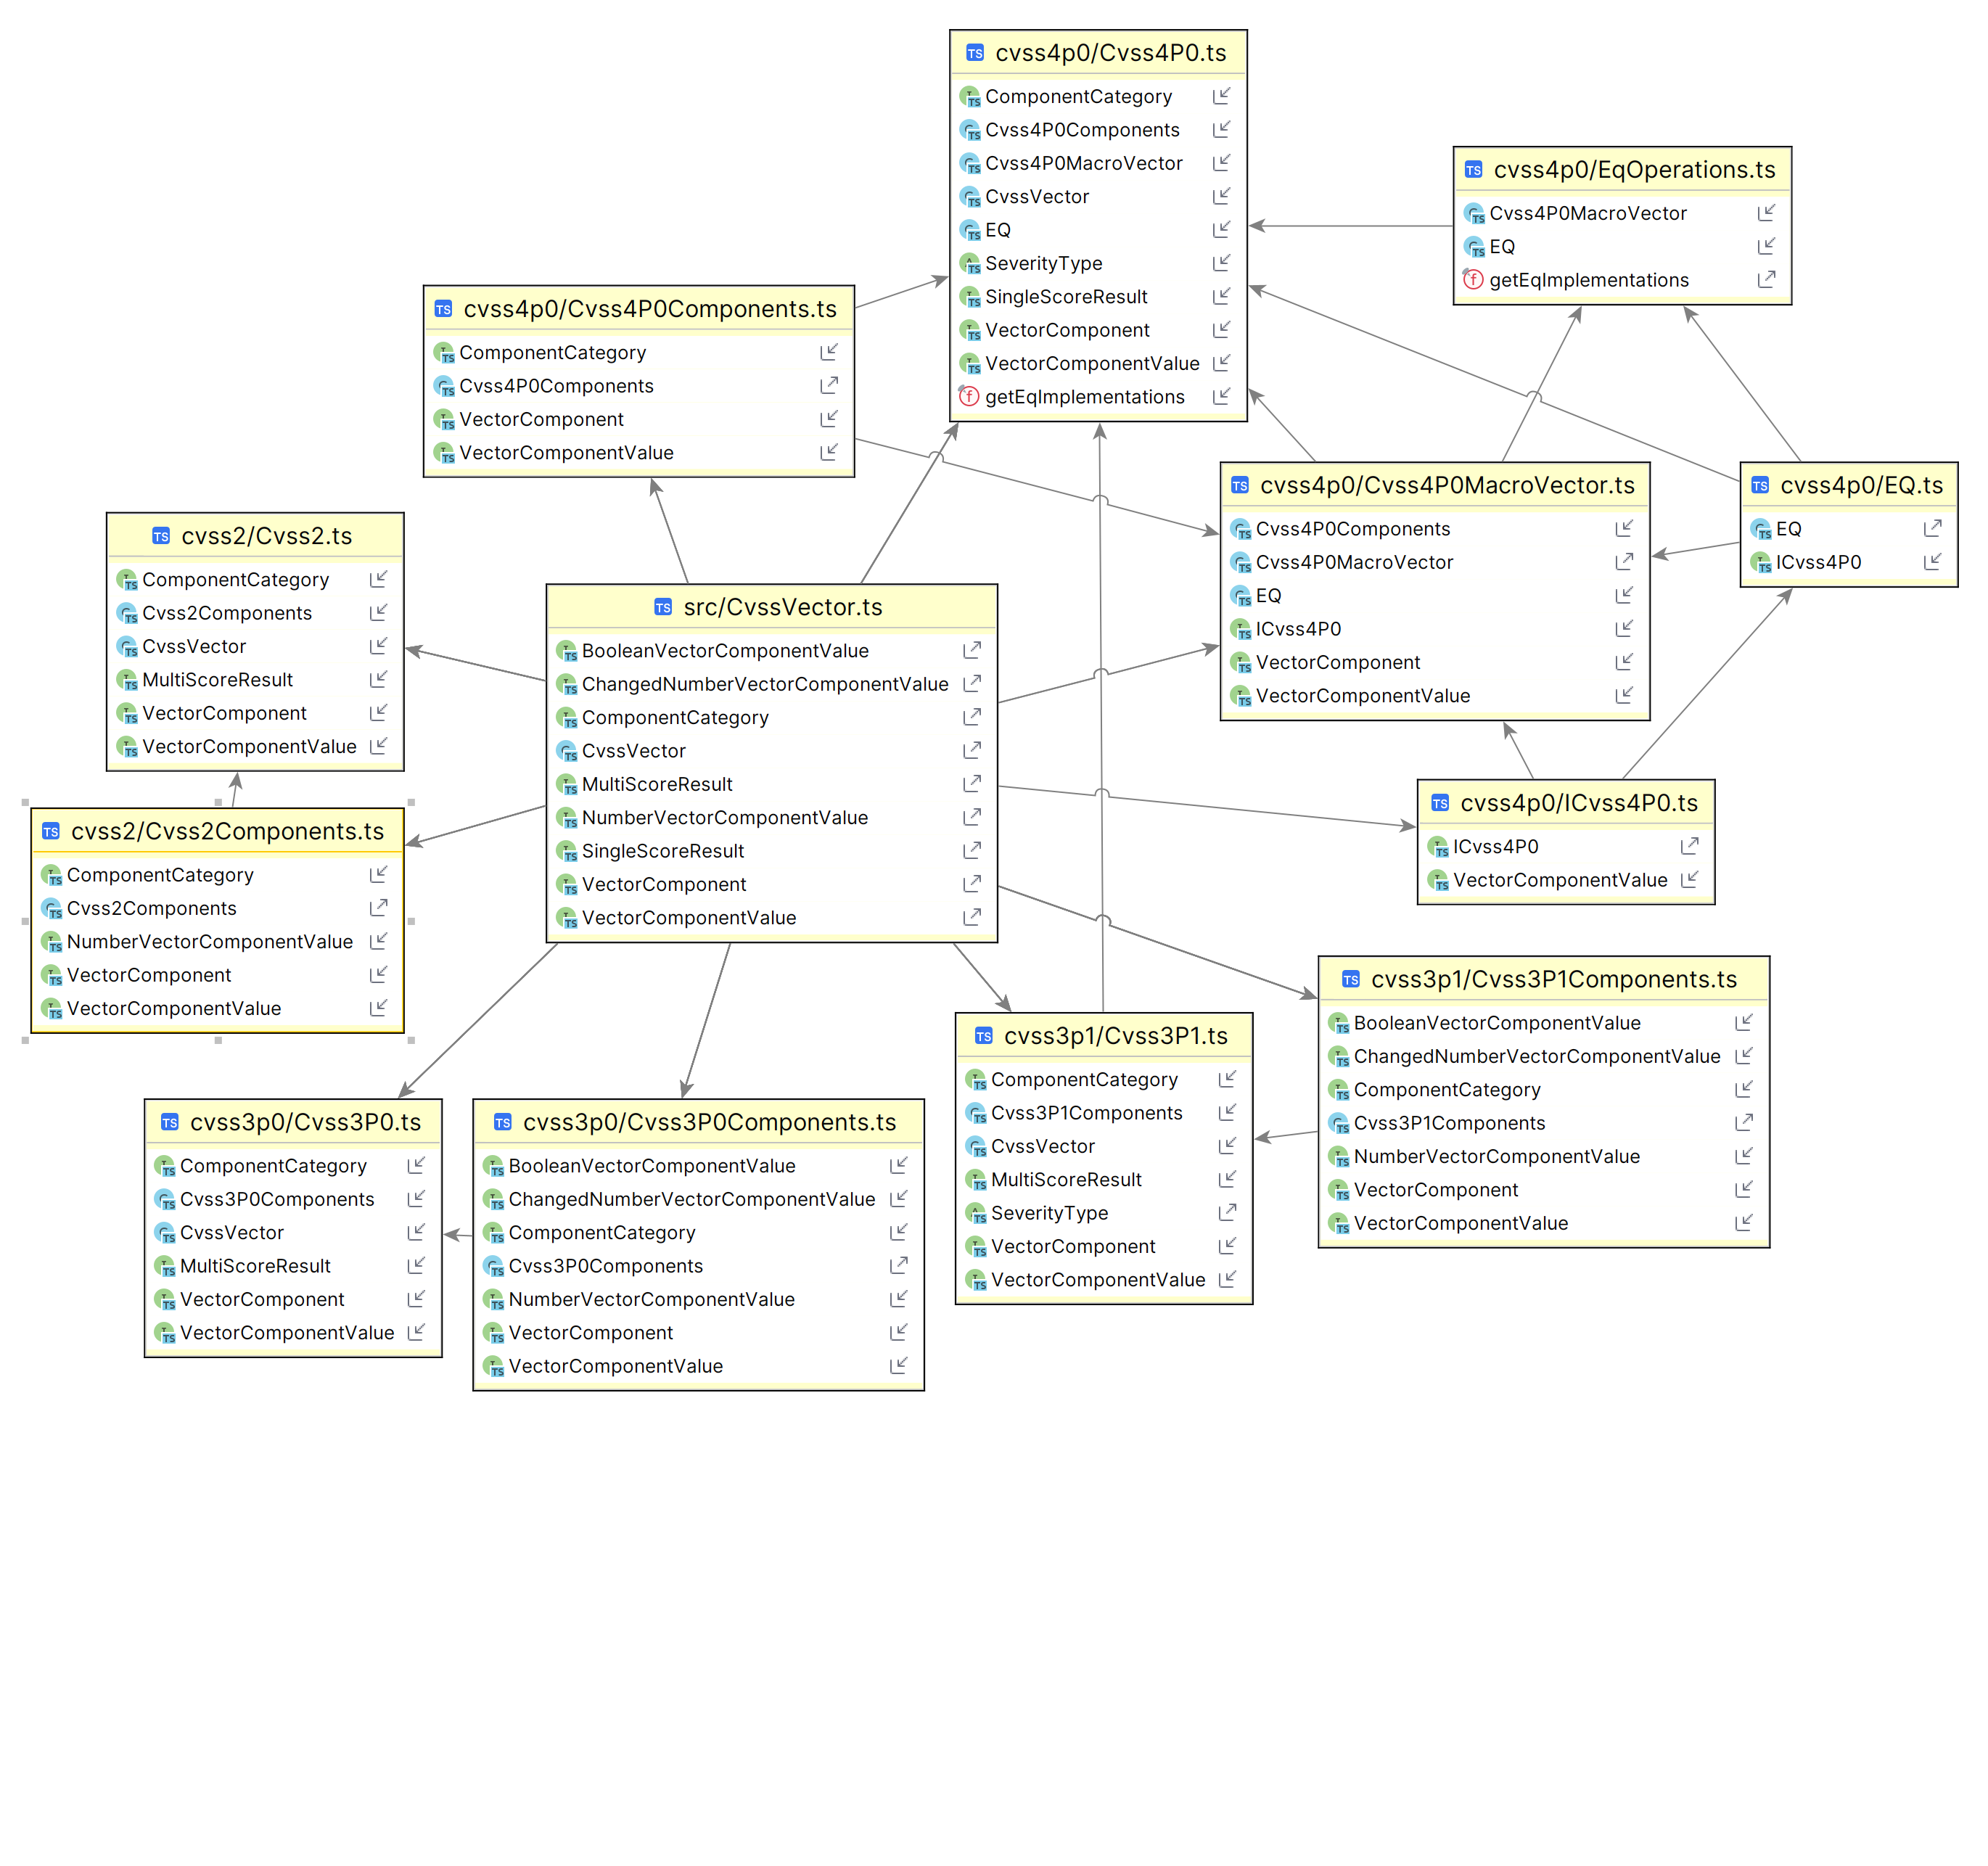
\includegraphics[width=1.0\textwidth, keepaspectratio]{res/grafiken/cvss-ts-calculator-class-diagram}}
    \caption{Klassendiagramm des CVSS-Rechners in TypeScript}
    \label{fig:cvss-ts-calculator-class-diagram}
\end{figure}

Da sich Vektor-Versionen nur in ihren verwendeten Metriken und der Score-Berechnung unterscheiden, kann recht viel der gemeinsamen Logik in die Oberklasse \code{CvssVector} (Ausschnitt in Listing \ref{lst:cvss-typescript-cvss-vector-class-attributes}) extrahiert werden.
Jede Vektor-Version definiert stark unterschiedliche Metriken, darum werden diese in der Klasse als beliebige Metriken in einer Map abgelegt.
Die Metriken von Vektoren der Versionen 2.0 und 3.1 müssen zudem aus der Spezifikation definierte Werte abspeichern, die für die Score-Berechnung verwendet werden.
Diese können unterschiedliche Datentypen haben, darum wird ein generischer Typ \code{VectorComponentValue} eingeführt, der Implementierungen wie \code{NumberVectorComponentValue} erlaubt.

\begin{lstlisting}[language=Java, label={lst:cvss-typescript-cvss-vector-class-attributes}, caption={Ausschnitt der CvssVector Klasse in TypeScript}, basicstyle=\scriptsize]
export abstract class CvssVector<R extends BaseScoreResult> {
    components: Map<VectorComponent<VectorComponentValue>, VectorComponentValue>;

    abstract calculateScores(normalize: boolean): R;
    abstract getVectorName(): string;
    setComponent(comp: VectorComponent<VectorComponentValue>, val: VectorComponentValue) { }
    getComponent<T extends VectorComponentValue>(comp: VectorComponent<T>): T { }
}
\end{lstlisting}

Die Methode \code{calculateScores} ist das Kernstück jeder Versionsimplementierung, in der immer ein Objekt mit mindestens einem Overall-Score und je nach Version zusätzliche Scores konstruiert und zurückgegeben wird.
In Listing \ref{lst:cvss-typescript-cvss-3P1-calculateScores} wird dies anhand von einigen Besonderheiten der Version 3.1 gezeigt:
CVSS 3.1 hat (unter anderem) das Problem, dass die sog. \qt{Environmental} und \qt{Temporal} Scores nicht von 0 bis 10 reichen, sondern nur bis 6.0 und 3.9.
Mit einem \code{normalize}-Parameter können diese Werte optional zur besseren Vergleichbarkeit mit anderen Versionen durch eine MapRange-Funktion auf die Spanne von 0 bis 10 überführt werden.\newline
Generell ist auch zu beachten, dass nicht immer kann jeder Score berechnet werden kann, denn natürlich müssen immer mindestens die zur Berechnung benötigten Metriken vorhanden sein.
Dies wird mit einfachen Abfragen auf die Existenz der Metriken überprüft, bevor die Score-Berechnungsmethoden aufgerufen werden.

\begin{lstlisting}[language=Java, label={lst:cvss-typescript-cvss-3P1-calculateScores}, caption={CVSS 3.1 Score-Berechnung in TypeScript}, basicstyle=\scriptsize]
calculateScores(normalize: boolean = false): MultiScoreResult {
    const base = isBaseFullyDefined();
    const temp = isAnyTemporalDefined();
    const env = isAnyEnvironmentalDefined();
    const result: MultiScoreResult = {};

    if (base) {
        result.base = round(base(), 1);
        result.impact = normalize(round(impact(), 1), normalize ? 6.0 : 10);
        result.exploitability = normalize(round(exploitability(), 1), normalize ? 3.9 : 10);
    }
    if (base && temp) {
        result.temporal = round(temporal(), 1);
    }
    if (base && env) {
        result.environmental = round(environmental(), 1);
        result.adjustedImpact = normalize(round(adjustedImpact(), 1), normalize ? 6.1 : 10);
    }
    return result;
}
\end{lstlisting}

Die CVSS-Spezifikation\footnote{\url{https://www.first.org/cvss/v3.1/specification-document\#CVSS-v3-1-Equations}} definiert die genauen Formeln und Methoden der Berechnungsmethoden, welche übernommen und in TypeScript implementiert wurden.
Ein typisches Beispiel dazu ist die Berechnung des CVSS 3.1 Impact-Scores, bei der auf diverse Metriken zugegriffen wird und diese mit weiteren im Standard definierten Konstanten verrechnet werden.
Hier kommen die unterschiedlichen Datentypen der Metriken zum Tragen, wie ein \code{boolean} für die Scope-Metrik oder \code{number} für die restlichen hier verwendeten.
Die dazugehörigen Formeln aus der Spezifikation werden hier und in Listing \ref{lst:cvss-typescript-cvss-3P1-calculateExactImpactScore} mit dem dazugehörigen Code abgebildet.
\begin{align*}
    \text{ISS} &= 1 - [ (1 - \text{Confidentiality}) \times (1 - \text{Integrity}) \times (1 - \text{Availability}) ] \\
    \text{If Scope is Unchanged:} & \quad 6.42 \times \text{ISS} \\
    \text{If Scope is Changed:} & \quad 7.52 \times (\text{ISS} - 0.029) - 3.25 \times (\text{ISS} - 0.02)^{15}
\end{align*}

\begin{lstlisting}[language=Java, label={lst:cvss-typescript-cvss-3P1-calculateExactImpactScore}, caption={CVSS 3.1 Impact Score-Berechnung in TypeScript}, basicstyle=\scriptsize]
public calculateExactImpactScore(): number {
    const iss = 1 - ((1 - getComponent(C).value)
                   * (1 - getComponent(I).value)
                   * (1 - getComponent(A).value));

    if (getComponent(S).value)
        return SCOPE_CHANGED_FACTOR * (iss - 0.029) - 3.25 * Math.pow(iss - 0.02, 15);
    else return SCOPE_UNCHANGED_FACTOR * iss;
}
\end{lstlisting}

\subsubsection{CVSS:4.0 TypeScript Implementierung} \label{subsec:projektbericht-loesungsweg-typescript-cvss-online-calculator-cvss-4P0}

Etwas anders verhält es sich mit der Version 4.0 von CVSS:
Diese definiert nur einen einzigen berechenbaren Score und verwendet zur Berechnung keine statischen Formeln wie in 2.0 und 3.1, sondern einige höhere mathematische Konzepte.
Diese Änderungen wurden bewusst getroffen:
Laut der Dokumentation und Entwicklungsgeschichte von CVSS 4.0 \cite{CVSSv4.0Specification} sollte nicht nur durch Reduktion auf einen einzigen Score die Interpretation der Ergebnisse vereinfacht (und Verwirrung reduziert) werden, sondern auch gegen die Kritik zu wirken, dass die Bildung der Scores in den Vorgängerversionen durch die recht abstrakten vordefinierten Formeln nicht intuitiv war.
Darum wurde für 4.0 ein anderer Ansatz gewählt.

Dazu wurden die 15 Millionen möglichen Vektoren dieser Version automatisiert von 32 Metrik-Dimensionen über diverse Regeln in einen nur 6-Dimensionalen Raum mit 270 sog.\ \qt{MakroVektoren} aufgeteilt, bei dem jede Dimension mit eigenen Regeln als eine \qt{Äquivalenzgruppe} bezeichnet wird.
Diese wurden einer Expertengruppe mit 50 Teilnehmern bereitgestellt, die diese je manuell dem Schweregrad in eine absolute Liste einordnen sollten.
Mit diesem Datensatz konnte eine durchschnittliche Liste an Vektoren mit aufsteigenden Schweregraden gebildet werden, die der aktuellen Meinung von Security-Experten gleicht, womit das Argument der Formel-Abstraktion entkräftet werden sollte.
Diesen abstrahierten Vektoren konnten dann recht einfach linear die CVSS-Scores von 0 bis 10 in einer Lookup-Tabelle statisch vergeben werden.

Um bei der Berechnung des Scores für einen initialen Input-Vektor diese Lookup-Tabelle verwenden zu können, muss daher der Vektor mit seinen 32 Metriken ebenso als erster Schritt auf nur 6 Dimensionen in einen MakroVektor reduziert werden.
Die 270 Scores der Lookup-Tabelle wären allerdings etwas wenig, um die Vielfalt und den Detailgrad aller 15 Millionen Kombinationen darzustellen.
Daher wird ein Interpolationschritt als zweiter Schritt dahinter geschaltet, der den Großteil der Berechnungslogik und der Komplexität einnimmt.

Die 6 Äquivalenzgruppen definieren jeweils einige Regeln, welche Metriken sie umfasst und wie sie zur Klassifizierung der Metriken beitragen.
In Listing \ref{lst:cvss-typescript-cvss-4P0-equivalence-groups} wird einmal die Klasse \code{EQ} und eine der Implementierungen zur zweiten Gruppe dazu gezeigt.
Sie repräsentieren effektiv die in der Spezifikation definierten Regeln und Funktionen\footnote{\url{https://www.first.org/cvss/v4.0/specification-document#CVSS-v4-0-Scoring-using-MacroVectors-and-Interpolation}}.

\begin{lstlisting}[language=Java, label={lst:cvss-typescript-cvss-4P0-equivalence-groups}, caption={CVSS 4.0 Äquivalenzgruppen in TypeScript}, basicstyle=\scriptsize]
class EQ {
    level: string;
    vectorDepth: number;
    highestSeverityVectors: ICvss4P0[] = [];
    predicate: (vector: ICvss4P0) => boolean;
}

public static EQ2_DEFINITIONS: EQ[] = [
    new EQ("0", 1, ["AC:L/AT:N"],
           vector => vector.get("AC") === "L" && vector.get("AT") === "N"),
    new EQ("1", 2, ["AC:H/AT:N", "AC:L/AT:P"],
           vector => !(vector.get("AC") === "L" && vector.get("AT") === "N"))
];
\end{lstlisting}

Auf diese beiden Schritte wird nun auf einem Niveau eingegangen, das einen Kompromiss zwischen Komplexität und Verständlichkeit erzielen soll.
Bevor auf die genauen Formeln eingegangen werden kann, müssen die zwei unterschiedlichen Skalen mit verschiedenen Bedeutungen erklärt werden:

\begin{description}
    \item[Severity Distance Scale] Diese Skala bezieht sich auf die Vektormetriken und deren möglichen Werten.
    Die kleinstmögliche Änderung von $\pm 1$ auf dieser Skala stellt eine Änderung eines einzelnen Metrikwerts um einen Wert nach oben oder unten dar ($+1$ = schwerer, $-1$ = weniger schwer).
    Da effektiv nur Distanzen zur oberen Grenze einzelner MakroVektoren berechnet werden, kann diese nur positive Werte annehmen.
    \item[CVSS Score Scale] Stellt als bereits genannte Skala des zu berechnenden Scores die Schwere der Schwachstelle in einem Bereich von 0 bis 10 dar, wobei höhere Werte auf schwerwiegendere Schwachstellen hinweisen.
    Die kleinste mögliche Änderung auf dieser Skala ist $0.1$.
\end{description}

\newpage
Die folgenden, zwar vollständig aus der Implementierung abgeleiteten Formeln, werden allerdings auf diese Weise nicht im Standard aufgeführt, da dieser sich eher mit den (mathematischen) Konzepten hinter der Berechnung beschäftigt und nicht mit den eigentlichen Berechnungsdetails.
Der gewünschte Score wird durch die Funktion \text{ScoreInterpolated}$(V)$ definiert.
\begin{align*}
    \text{ScoreInterpolated}(V) &= \text{ScoreBase}(MV) - \text{Mean}(\text{ScoreEQ(EQ1)}, ..., \text{ScoreEQ(EQ6)}) \\
    \text{ScoreEQ}(EQ) &= \text{ProportionDistance}(V, EQ) \times \text{ScoreRange}(MV, EQ) \\
    \text{ProportionDistance}(V, EQ) &= \frac{\text{SeverityDistance}(V, \text{MV})}{\text{Depth}(\text{MV})}
\end{align*}

Damit können die folgenden Werte und Formeln definiert werden:

\begin{itemize}[noitemsep]
    \item \textbf{MV} stellt den aus dem ursprünglichen Vektor berechneten MakroVektor dar.
    \item \textbf{EQ} wird mit einer Sammlung an Definitionen und Funktionen als sog.\ Äquivalenzgruppe bezeichnet, die definieren, wann eine Metrik-Untermenge eines Vektors einer Gruppe entspricht und führen je eine Liste der höchsten Schwerevektoren die ihren Kriterien entsprechen.
    \item \textbf{ScoreInterpolated$(V)$} ist das Ziel der Berechnung, der finale Score für den Vektor.
    Sie kombiniert den Basis-Score mit den durchschnittlichen Anpassungen durch die Äquivalenzgruppen.
    \item \textbf{ScoreBase$(MV)$} durch Nachschlagen in der Lookup-Tabelle erhaltener Basis-Score.
    \item \textbf{Mean$(scores)$} (CVSS Score Scale) berechnet den Durchschnittsscore über alle EQ-Gruppen, die für den Vektor zutreffen.
    Nicht immer kann eine EQ für einen Vektor berechnet werden.
    \item \textbf{ScoreEQ}(EQ) (CVSS Score Scale) berechnet eine für die aktuelle EQ-Gruppe proportionale Score-Anpassung.
    Diese wird berechnet durch Multiplikation eines Wertes zwischen 0 und 1 (siehe \text{ProportionDistance}) und der Score Range, also welche maximale Score-Differenz innerhalb der EQ-Gruppe möglich ist.
    \item \textbf{ProportionDistance$(V, EQ)$} ist ein Wert zwischen 0 und 1 (0-100\%) und definiert, wie weit der Vektor von der höchsten Schwere innerhalb der EQ-Gruppe entfernt ist, in Bezug auf den gesamten Schwerebereich des MakroVektors.
    \item \textbf{SeverityDistance$(V, MV)$} (Severity Distance Scale) ist die Anzahl der Metrikwertänderungen, die benötigt werden, um den Vektor $V$ vom Vektor mit der höchsten Schwere innerhalb desselben MacroVectors zu erreichen.
    \item \textbf{Depth$(MV)$} (Severity Distance Scale) ist die Gesamtanzahl der Metrikwertänderungen innerhalb eines MacroVectors von seinem niedrigsten bis zu seinem höchsten Schwerevektor.
    Diese ist je nach MakroVektor unterschiedlich, da jeder unterschiedlich breit sein kann.
    \item \textbf{ScoreRange$(MV, EQ)$} (CVSS Score Scale) ist der maximale Unterschied im Score zwischen dem höchsten und niedrigsten Schwerevektor innerhalb des MacroVectors für eine gegebene EQ-Gruppe.
    Sie repräsentiert die effektive Score-Spanne innerhalb eines MakroVektors.
\end{itemize}

\newpage
In Listing \ref{lst:cvss-typescript-cvss-4P0-calculateOverallScore-pseudocode} wird nun ein Pseudocode für die Berechnung des Scores gezeigt, wie er ausgeprägt als TypeScript Code in der Cvss4P0-Klasse gefunden werden kann.

\begin{lstlisting}[language=Python, label={lst:cvss-typescript-cvss-4P0-calculateOverallScore-pseudocode}, caption={CVSS 4.0 Score-Berechnung Pseudocode}, basicstyle=\scriptsize]
function calculateScore(vector):
  if not baseDefined(vector) or noImpact(vector):
      return 0.0

  # encapsulated implementations for equivalence groups handling
  eqGroups = getEquivalenceGroups()

  macro = getMacroVector(vector)
  baseScore = lookupTableScore(macro)

  # collect vectors with highest severity from each equivalence group
  highestSevVectors = [group.getSevereVectors(macro) for group in eqGroups]

  # since each group may have multiple highest vectors, generate all permutations
  combinations = generateCvssPermutations(highestSevVectors)
  if combinations.isEmpty():
      return 0.0 # no max vectors found, does not happen in practice

  # the severity distances for all metrics between each combination and the input vector are
  # calculated. the first permutation with a combined positive severity distance is selected.
  for combination in combinations:
       severityDistances = calculateSeverityDistances(combination) # map<metric, distance>
       if sum(severityDistances) > 0:
           break

  # calculate the average of all proportional adjustments for all applicable groups
  adjustment = AverageCalculator()
  for group in eqGroups:
      lessSevereMacro = group.nextLowerMacro(macro)
      lowerScore = group.lookupScoresForNextLowerMacro(lessSevereMacro)
      # lowerScore is NaN if the current macro's group is already the lowest,
      # leading to availableSeverityReduction also potentially becoming NaN
      availableSeverityReduction = baseScore - lowerScore

       # all depth values are precalculated and defined by the specification
      depth = group.macroDepth(macro)
      distanceToHighest = sum(group.filterRelevantMetrics(severityDistances))

      # NaN is purposefully used as an indicator by the specification
      if not isNaN(availableSeverityReduction) and depth != 0.0:
          distancePercentageToNext = distanceToHighest / depth
          normalizedDistance = distancePercentageToNext * availableSeverityReduction
          adjustment.add(normalizedDistance)

  adjustedScore = baseScore - adjustment.averageOrDefault(0)
  return adjustScoreRange(adjustedScore)
\end{lstlisting}
